\FILE{section/eq-result.tex}

\subsection{Earthquake Result}

While using this framework we have conducted a parameter study for earthquake forecasting. Figure \ref{fig:eq1} and \ref{fig:eq2} show the results of this application. A more in depth paper about this application has been published in \cite{las-2023-mlcommons-edu-eq}, \cite{las-2023-escience} and \cite{las-2023-ai-workflow}.

\begin{figure*}[p]
     \centering
     \begin{subfigure}[b]{0.49\textwidth}
        \centering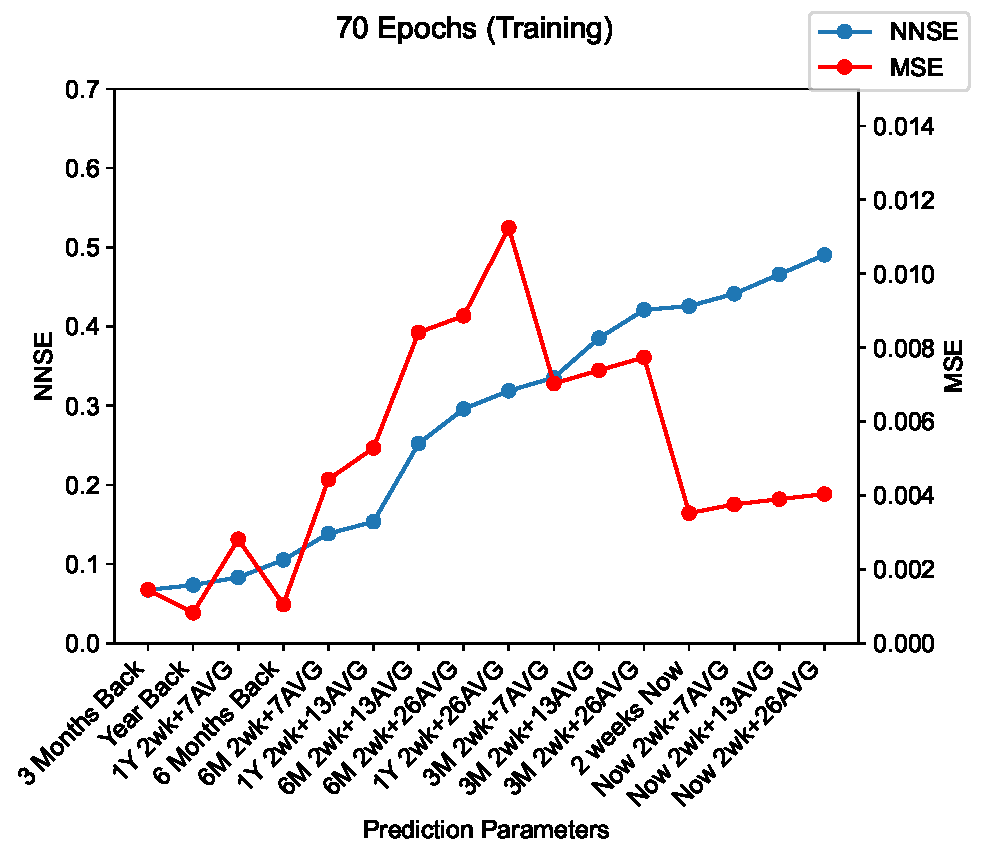
\includegraphics[width=1.0\linewidth]{images/70_training-MSE-and-NNSE.pdf}
        \caption{MSE and NNSE - 70 epochs training}
        \label{fig:eq1}
     \end{subfigure}
     \hfill
     \begin{subfigure}[b]{0.49\textwidth}
        \centering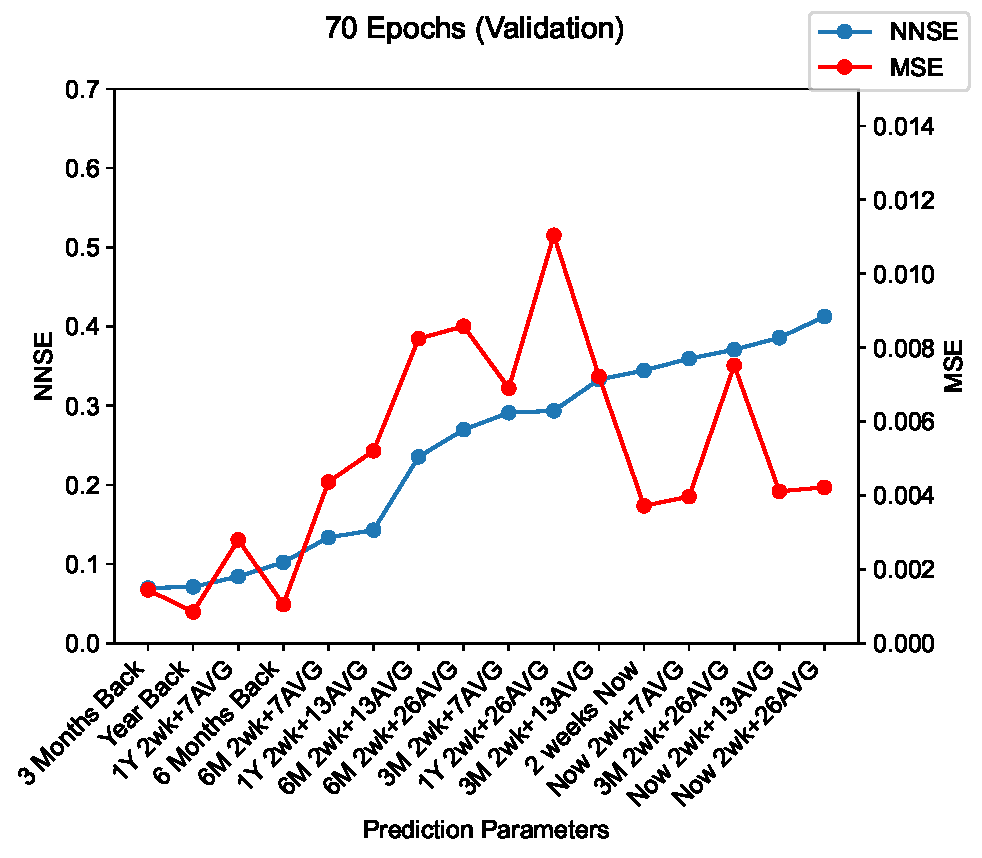
\includegraphics[width=1.0\linewidth]{images/70_validation-MSE-and-NNSE.pdf}
        \caption{MSE and NNSE - 70 epochs validation}
        \label{fig:tbd4}
     \end{subfigure}
        \caption{NNSE and MSE values for 70 epochs 70 (training and validation).}
        \label{fig:eq2}
\end{figure*}
